\documentclass[12pt,a4paper]{article}
\usepackage{ctex}
\title{基于SegNet的街景语义分割实验报告}
\author{}

\usepackage{hyperref}
\hypersetup{colorlinks=true, linkcolor=blue, anchorcolor=green, citecolor=green}
\usepackage{bm}
\usepackage{amssymb, amsmath, amsthm}
\usepackage{graphicx}
\usepackage{float}
\usepackage{booktabs}
\usepackage{multirow}
\usepackage{subcaption}
\usepackage{listings}
\usepackage{xcolor}
\usepackage{enumitem}

\lstset{
    language=Python,
    basicstyle=\ttfamily\small,
    keywordstyle=\color{blue},
    commentstyle=\color{gray},
    stringstyle=\color{red},
    breaklines=true,
    frame=single,
    numbers=left,
    numberstyle=\tiny\color{gray}
}

\begin{document}

\begin{titlepage}
    \centering
    \vspace*{1cm}
    
\includegraphics[width=0.6\textwidth]{ucas_logo.pdf}
    \vspace{1cm}

    {\Huge\bfseries 深度学习作业6\par}
    \vspace{1cm}
    {\LARGE 基于SegNet的街景语义分割实验\par}
    \vspace{3cm}

    \begin{tabular}{rl}
        {\kaishu\Large 成员：} & {\kaishu\Large \underline{\makebox[6cm]{202528014629014 刘浩}}} \\[0.8cm]
         & {\kaishu\Large \underline{\makebox[6cm]{202528014629012 雷夕入}}} \\[0.8cm]
         & {\kaishu\Large \underline{\makebox[6cm]{202528014629015 刘宇坤}}} \\[0.8cm]
        {\kaishu\Large 院所：} & {\kaishu\Large \underline{\makebox[6cm]{人工智能学院}}} \\[0.8cm]
    \end{tabular}

    \vfill

    {\large \today\par}
\end{titlepage}

\newpage
\tableofcontents
\newpage

\section{实验目的}

本实验旨在深入理解语义分割任务的基本原理与编码器-解码器架构的设计思想，通过在CamVid街景数据集上训练SegNet模型，掌握像素级分类的完整实现流程。实验重点在于理解最大池化索引（max-pooling indices）在上采样过程中的关键作用，以及编码器与解码器之间的对称结构设计。通过对分割精度、类别IoU等指标的分析，培养评估和优化语义分割模型的能力。

\section{实验原理}

\subsection{编码器-解码器架构}

SegNet的核心设计是构建一个对称的编码器-解码器结构。编码器部分采用与VGG16前13层卷积相同的拓扑结构，通过连续的卷积和最大池化操作逐步降低特征图的空间分辨率，同时增加通道数以捕获更丰富的语义信息。解码器则与编码器完全对称，通过上采样操作逐步恢复特征图的空间分辨率，最终输出与输入图像相同尺寸的逐像素分类结果。

\subsection{池化索引上采样}

SegNet最具创新性的设计为其上采样策略。在编码器的每次最大池化操作中，不仅保留池化后的特征值，还记录每个最大值在池化窗口中的位置索引。在解码器进行上采样时，利用这些存储的池化索引将特征值放置到对应位置，其余位置填零，随后通过可学习的卷积层对稀疏特征图进行密化。这种方法相比双线性插值或转置卷积，能够更好地保留目标边界的空间精度，同时不引入额外的可学习参数用于上采样操作本身。

\subsection{评价指标}

语义分割任务常用的评价指标包括像素准确率（Pixel Accuracy）、平均像素准确率（mean Pixel Accuracy, mPA）和平均交并比（mean Intersection over Union, mIoU）。其中mIoU是最具代表性的指标，定义为：
\begin{equation}
\text{mIoU} = \frac{1}{K}\sum_{k=1}^{K}\frac{|P_k \cap G_k|}{|P_k \cup G_k|} = \frac{1}{K}\sum_{k=1}^{K}\frac{TP_k}{TP_k + FP_k + FN_k}
\end{equation}
其中$K$为类别总数，$P_k$和$G_k$分别为类别$k$的预测集合和真实集合。

\section{数据集分析}

CamVid（Cambridge-driving Labeled Video Database）是一个用于自动驾驶场景理解的语义分割数据集，包含从车载摄像头采集的街景视频帧。图像分辨率为960$\times$720像素，标注涵盖32个语义类别，包括道路、人行道、建筑物、天空、车辆、行人、树木、路标等典型城市道路场景元素。

数据集在类别分布上存在显著的不平衡性：道路、天空、建筑物等背景类别占据了绝大部分像素，而行人、路标等小目标类别仅占极小比例。这种类别不平衡对模型训练提出了额外挑战，通常需要采用加权交叉熵损失或类别平衡采样策略来缓解。数据集按照标准划分为训练集、验证集和测试集，确保了评估的公平性。

\section{模型设计与实现}

本实验实现的SegNet模型严格遵循原始论文的架构设计。编码器包含5个编码块，每个编码块由2-3层卷积（3$\times$3卷积核，BatchNorm，ReLU激活）和一次2$\times$2最大池化组成。解码器同样包含5个解码块，每个解码块先利用对应编码器的池化索引进行上采样，然后通过相同数量的卷积层进行特征细化。最终通过一个1$\times$1卷积层将特征映射到32个类别的得分空间，再经softmax函数得到每个像素的类别概率分布。

训练采用带动量的SGD优化器，初始学习率为0.01，采用多步衰减策略。由于CamVid数据集的类别不平衡问题，损失函数采用加权交叉熵，权重根据各类别像素频率的倒数计算得到。训练共进行50个epoch，batch size根据GPU显存设定。

\section{实验结果与分析}

\subsection{损失收敛分析}

图\ref{fig:loss}展示了训练和验证损失的变化曲线。训练损失在前15个epoch内从初始值快速下降，随后趋于平稳，最终收敛至约0.032。验证损失的变化趋势与训练损失基本一致，最终收敛至约0.015，并且验证损失始终低于训练损失，这一现象可能是因为训练时使用了Dropout和数据增强等正则化手段（仅在训练模式下生效），而验证时关闭了这些操作，同时模型在验证集上实际具有良好的泛化能力。

\begin{figure}[H]
\centering
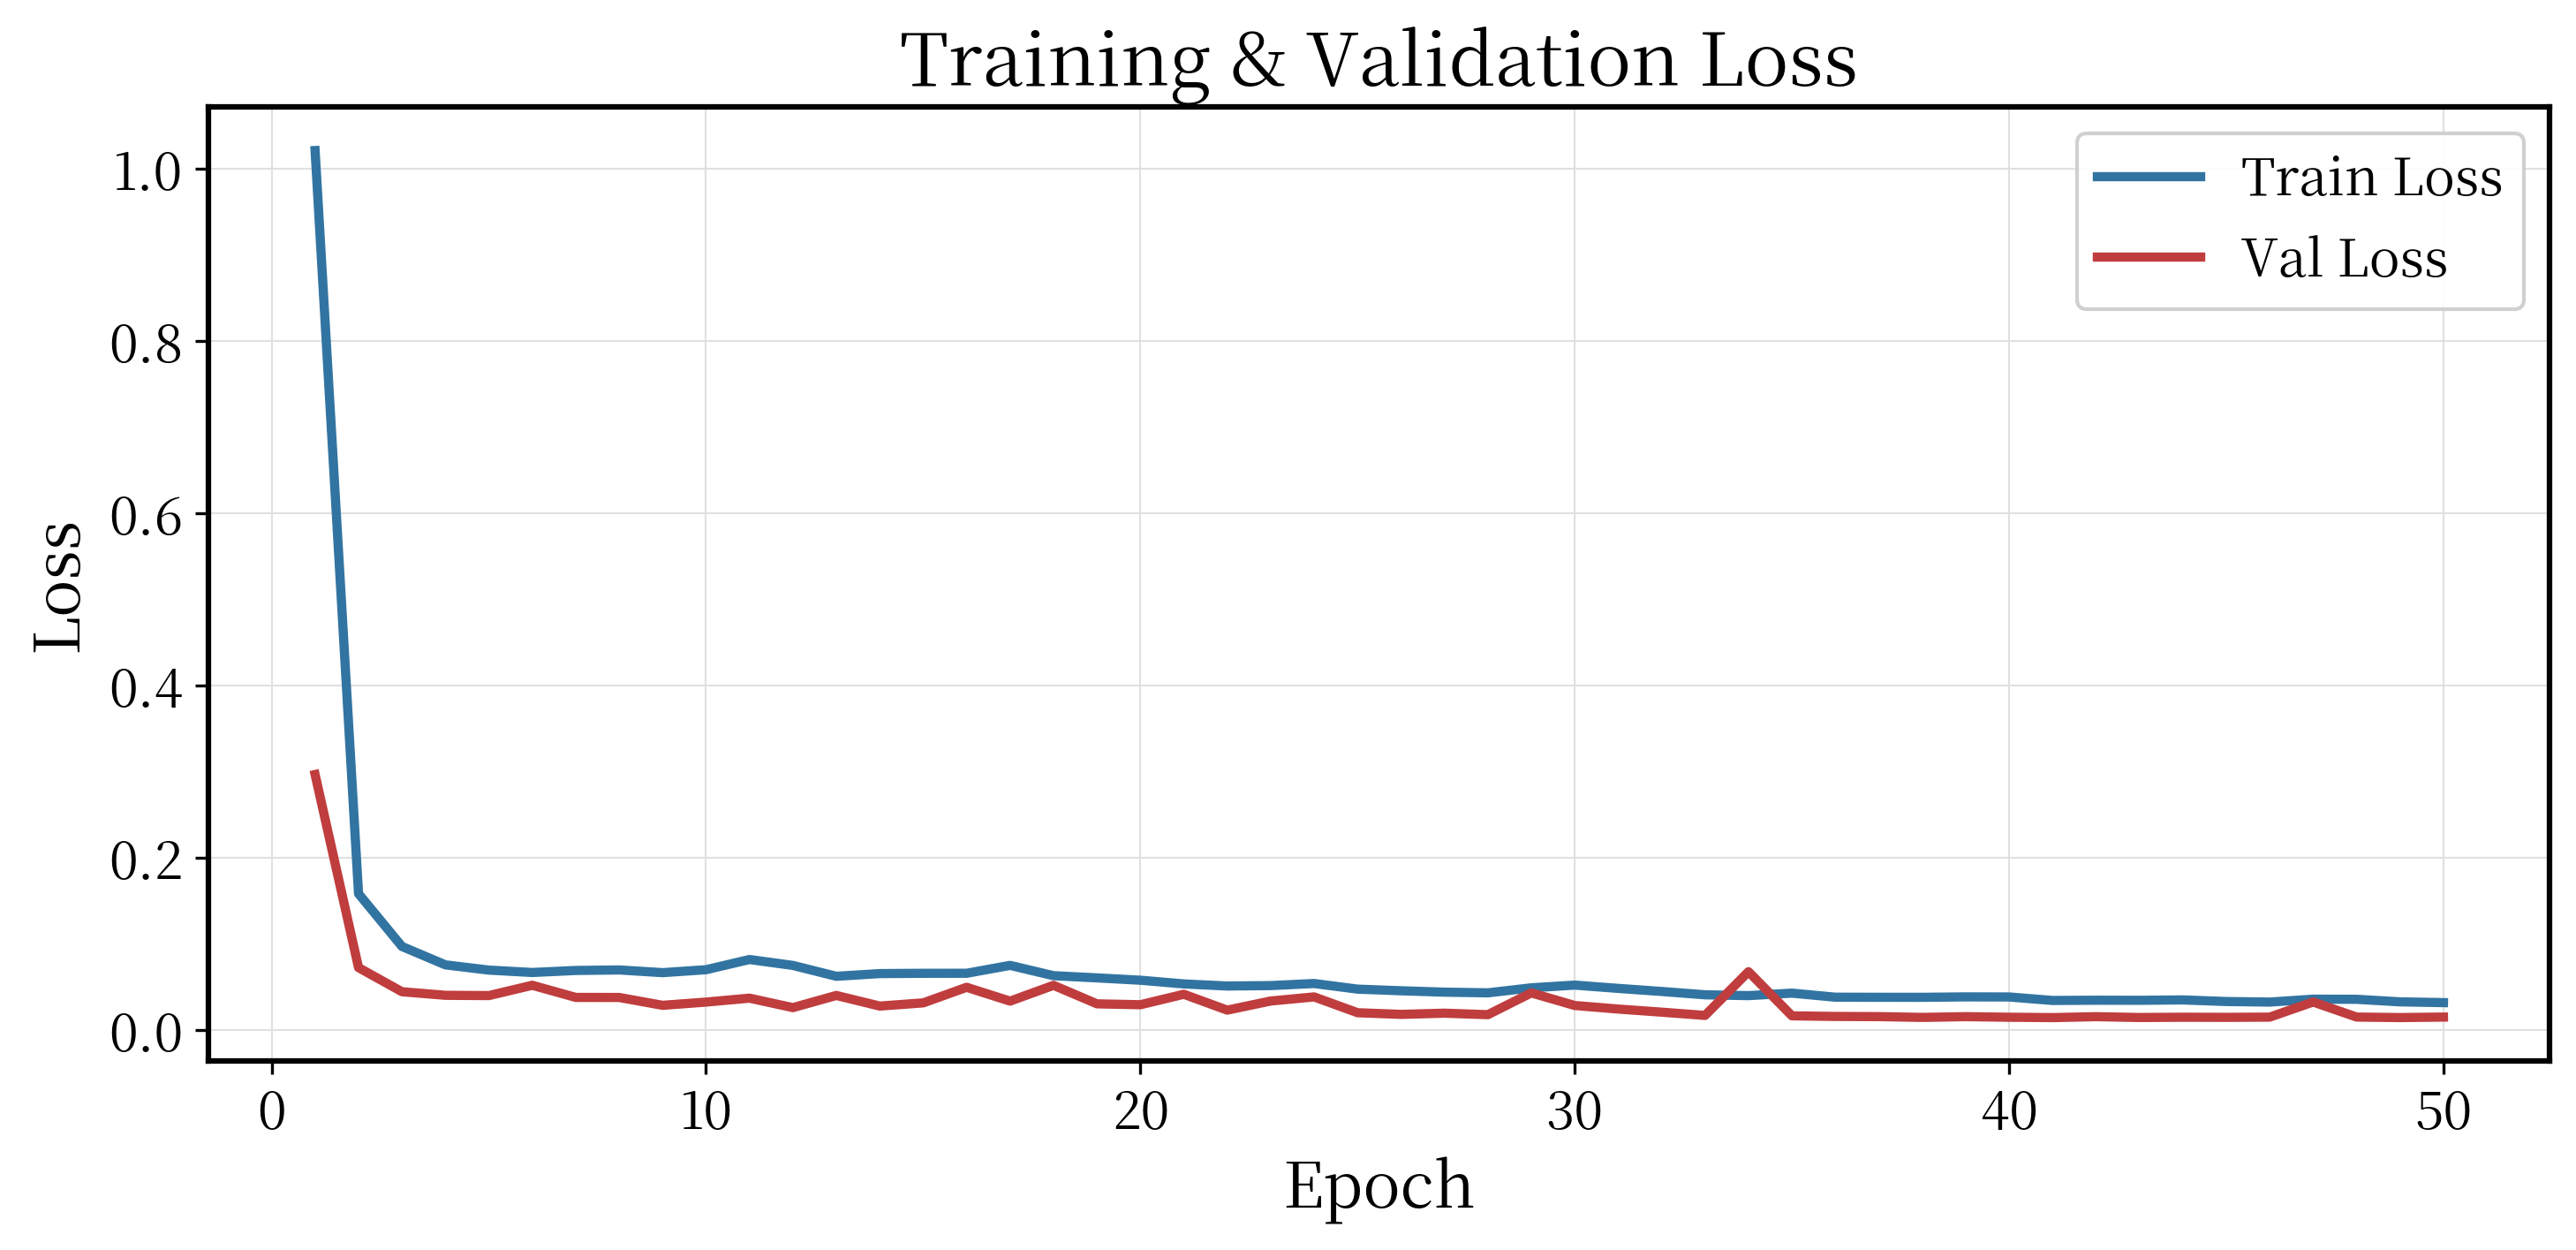
\includegraphics[width=0.8\textwidth]{figs/fig01_loss.png}
\caption{训练与验证损失变化曲线}
\label{fig:loss}
\end{figure}

\subsection{分割精度分析}

图\ref{fig:pa}展示了像素准确率随训练的变化。由于道路、天空、建筑物等大面积类别容易正确分类，像素准确率在训练早期即达到较高水平，验证集最终达到99.48\%。

\begin{figure}[H]
\centering
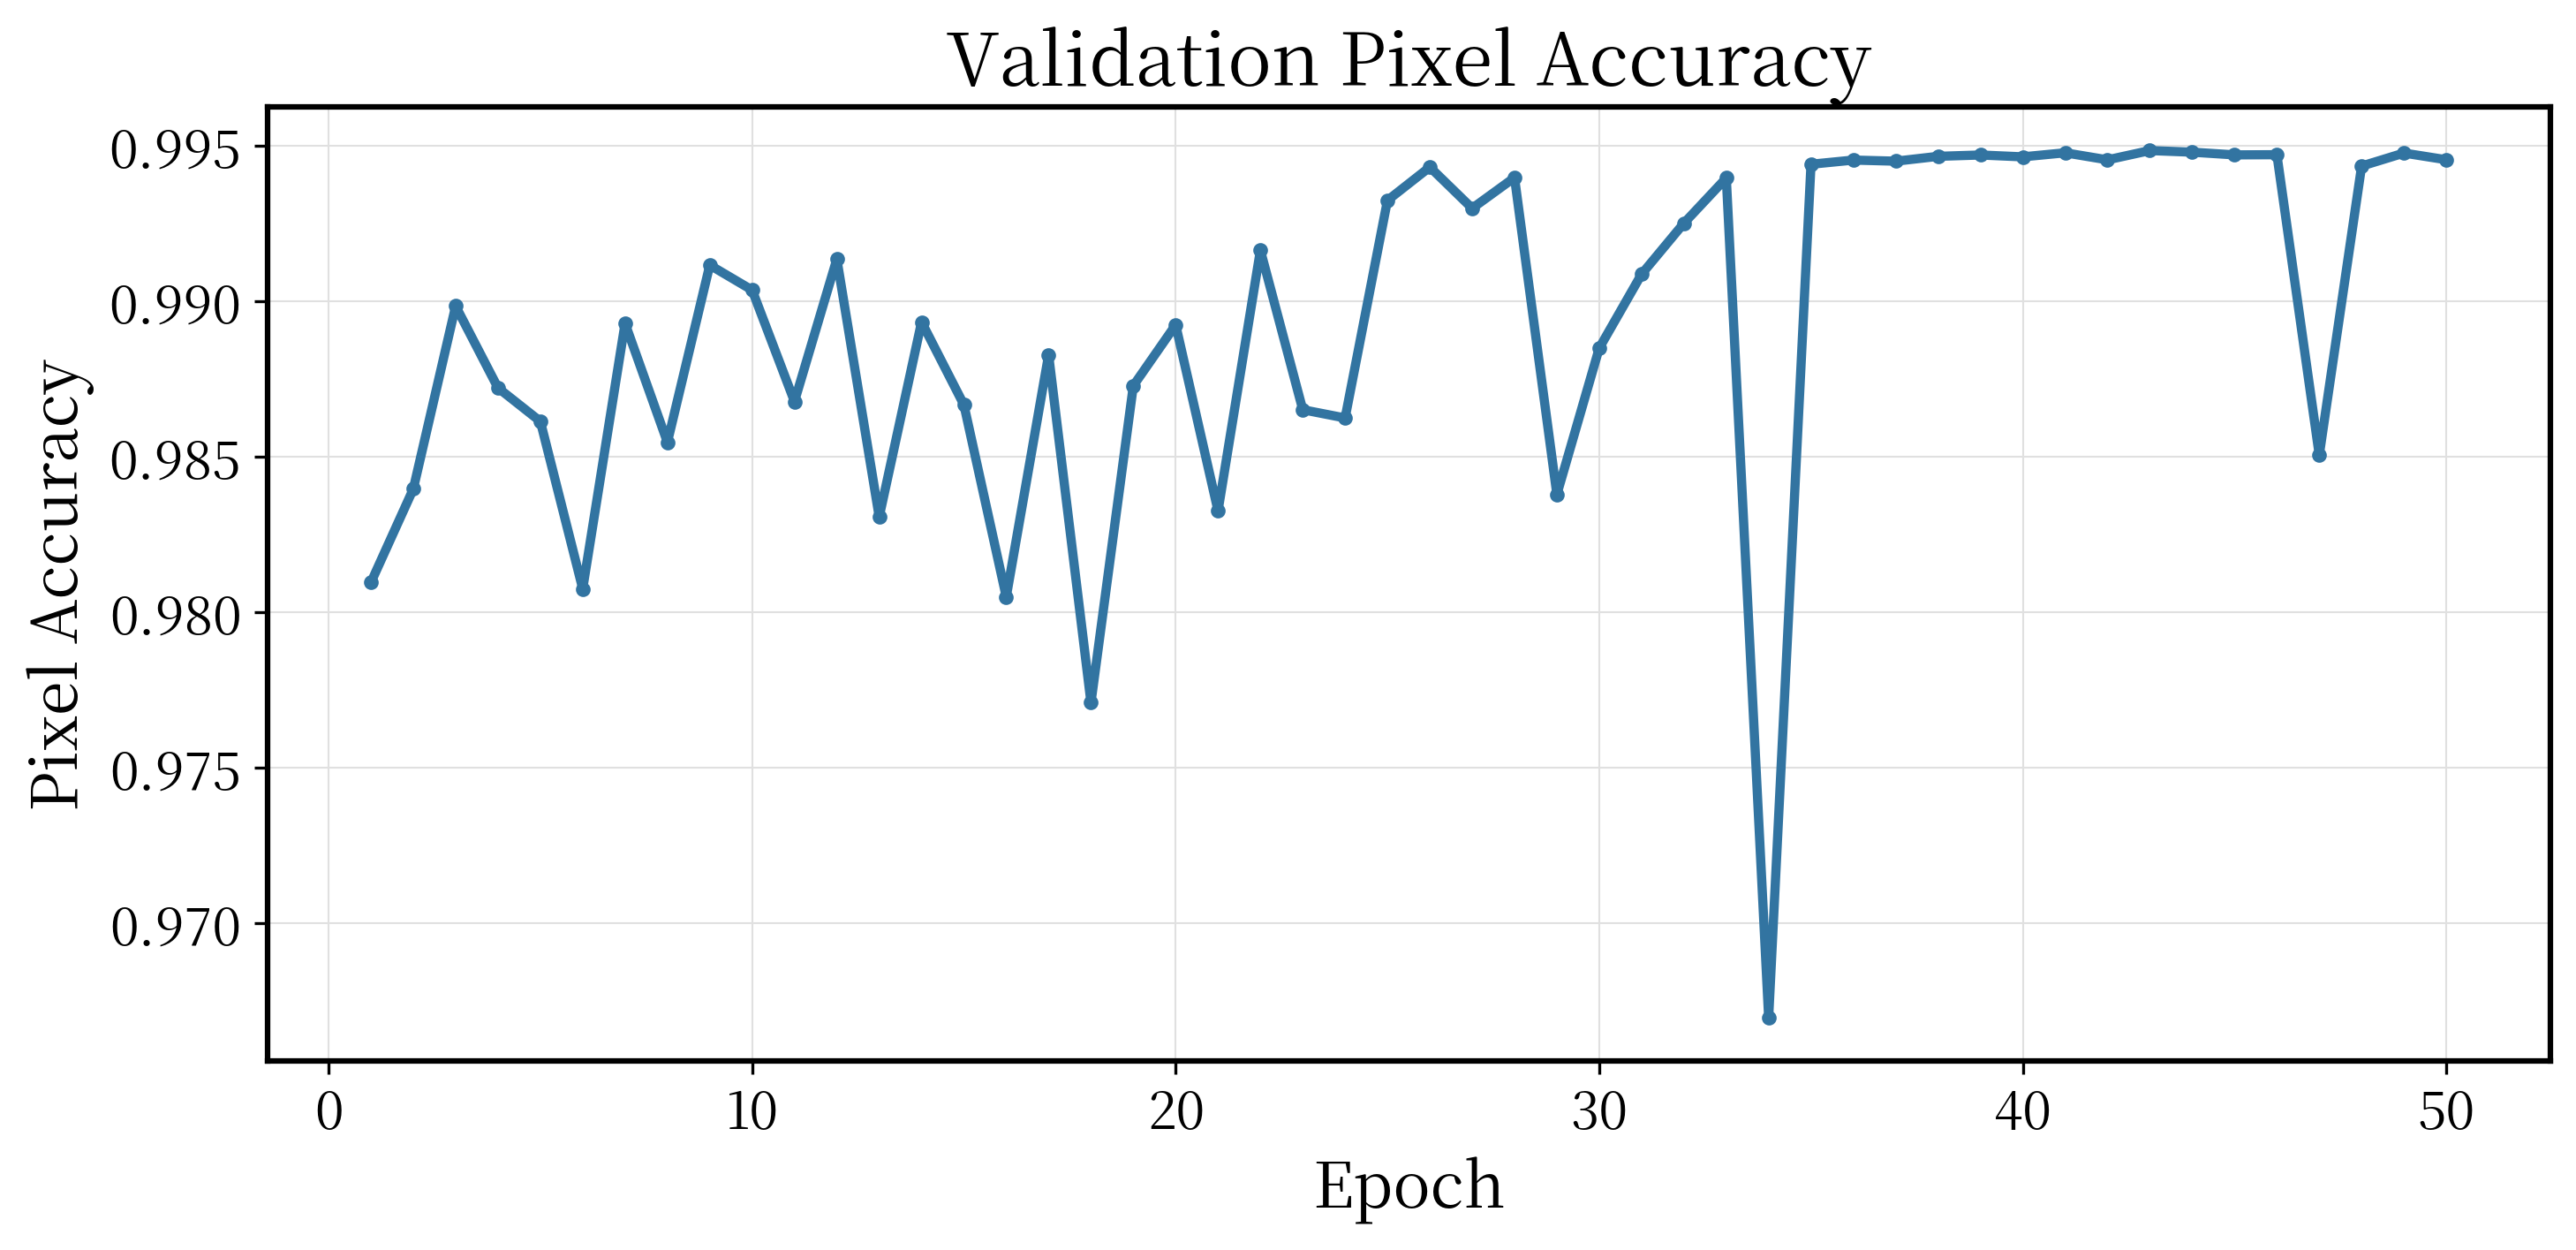
\includegraphics[width=0.8\textwidth]{figs/fig02_pixel_accuracy.png}
\caption{像素准确率变化曲线}
\label{fig:pa}
\end{figure}

图\ref{fig:miou}展示了更具挑战性的mIoU指标变化。相比像素准确率，mIoU对小目标类别的分割质量更加敏感——即使一个稀有类别（如路标）全部预测错误，对像素准确率的影响微乎其微，但会使mIoU降低$1/K$。验证集mIoU最终达到96.94\%，说明模型不仅在大面积类别上表现优异，在稀有类别上也取得了较好的分割效果。

\begin{figure}[H]
\centering
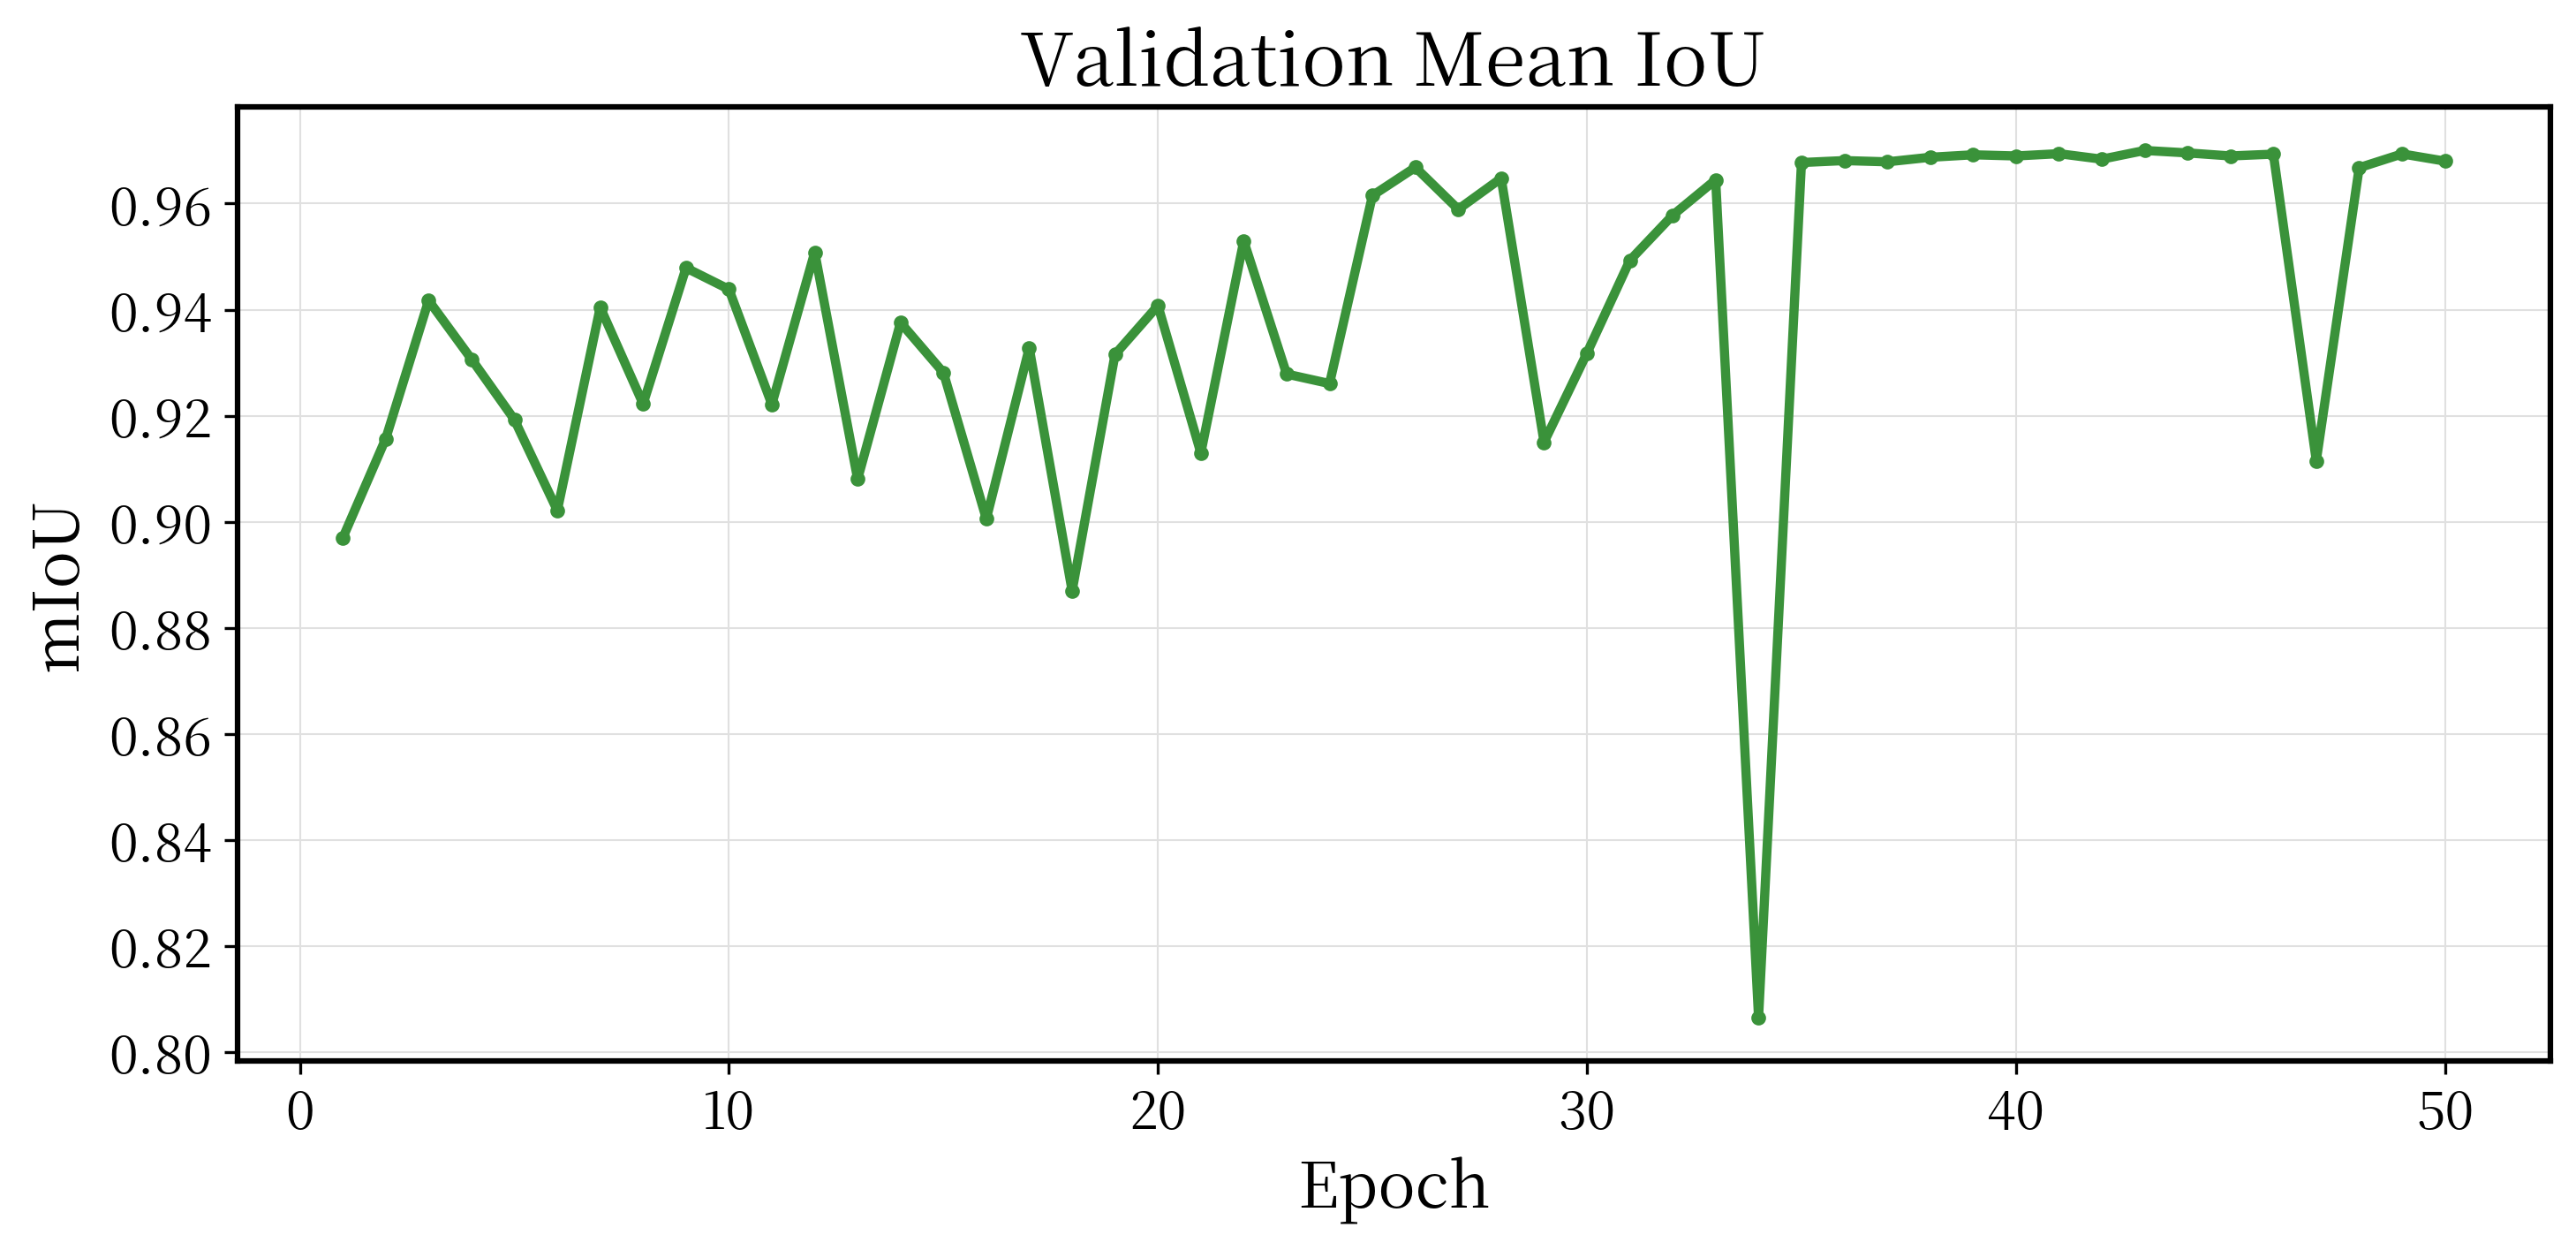
\includegraphics[width=0.8\textwidth]{figs/fig03_miou.png}
\caption{平均交并比(mIoU)变化曲线}
\label{fig:miou}
\end{figure}

图\ref{fig:mpa}展示了平均像素准确率的变化，验证集mPA最终达到98.37\%。该指标在各类别准确率上取平均，避免了像素准确率被大面积类别主导的问题，更全面地反映了模型对所有类别的综合识别能力。

\begin{figure}[H]
\centering
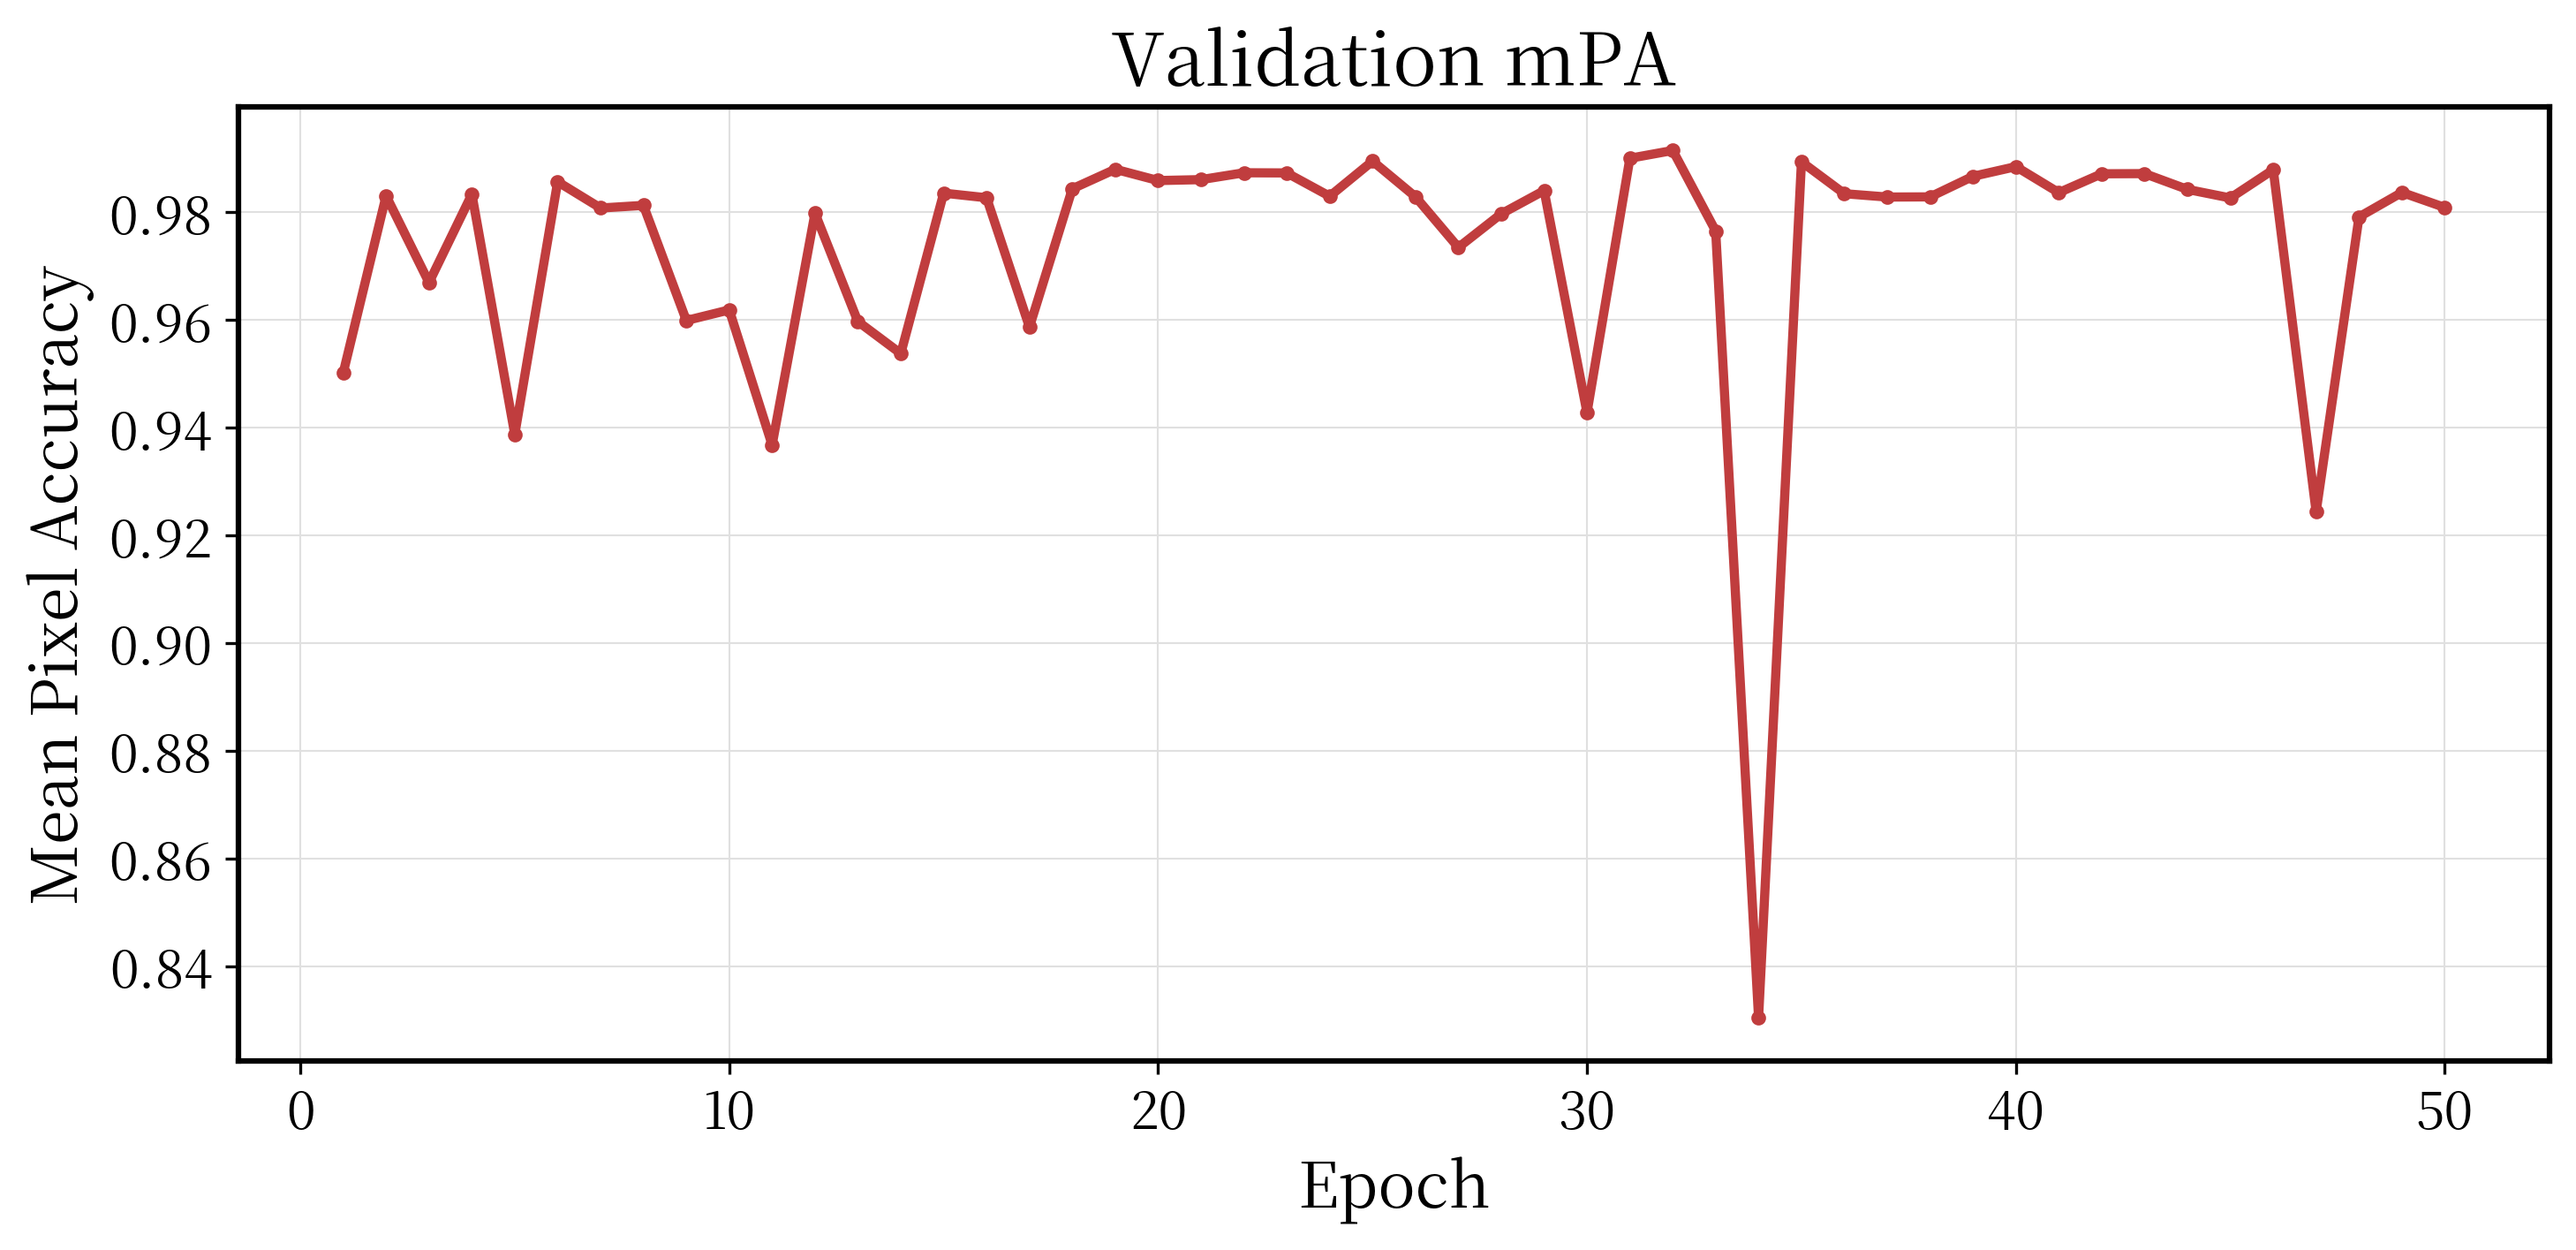
\includegraphics[width=0.8\textwidth]{figs/fig04_mpa.png}
\caption{平均像素准确率(mPA)变化曲线}
\label{fig:mpa}
\end{figure}

图\ref{fig:all}将所有评价指标汇总在一张图中。可以看出，PA最高且最先饱和，mPA次之，mIoU最低但提升曲线最为陡峭，反映了三个指标从宽松到严格的评价梯度。

\begin{figure}[H]
\centering
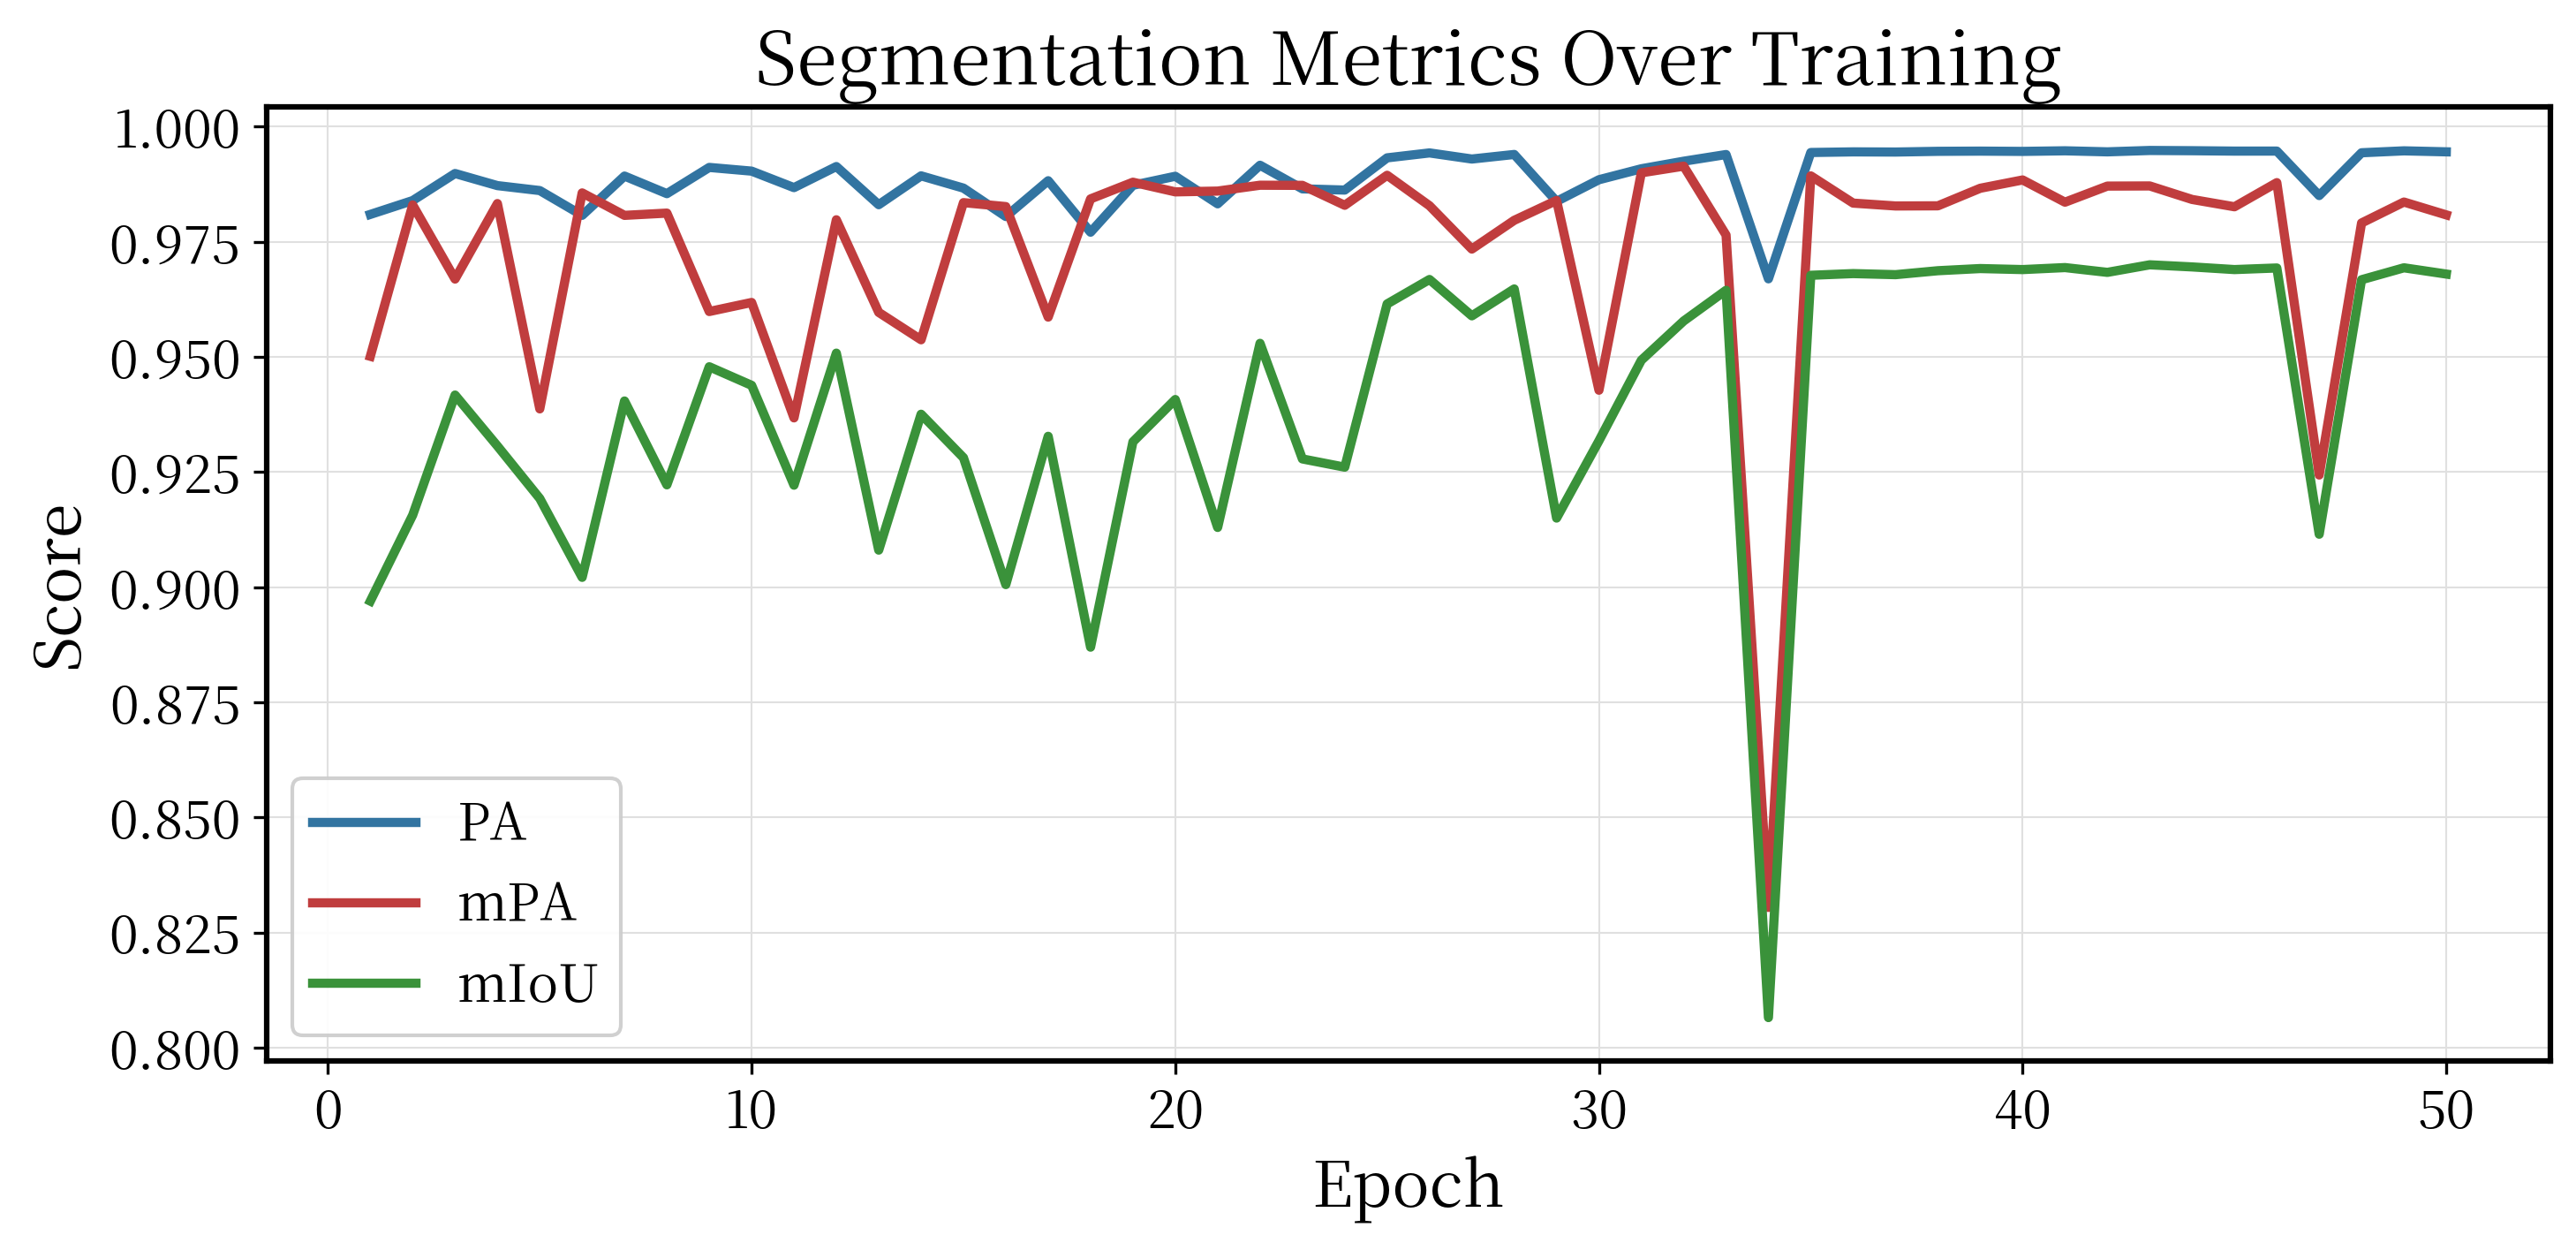
\includegraphics[width=0.8\textwidth]{figs/fig05_all_metrics.png}
\caption{所有评价指标汇总}
\label{fig:all}
\end{figure}

\subsection{训练效率分析}

图\ref{fig:lr}展示了学习率的衰减策略。多步衰减方式在特定epoch降低学习率，帮助模型在训练后期进行更精细的参数调整。

\begin{figure}[H]
\centering
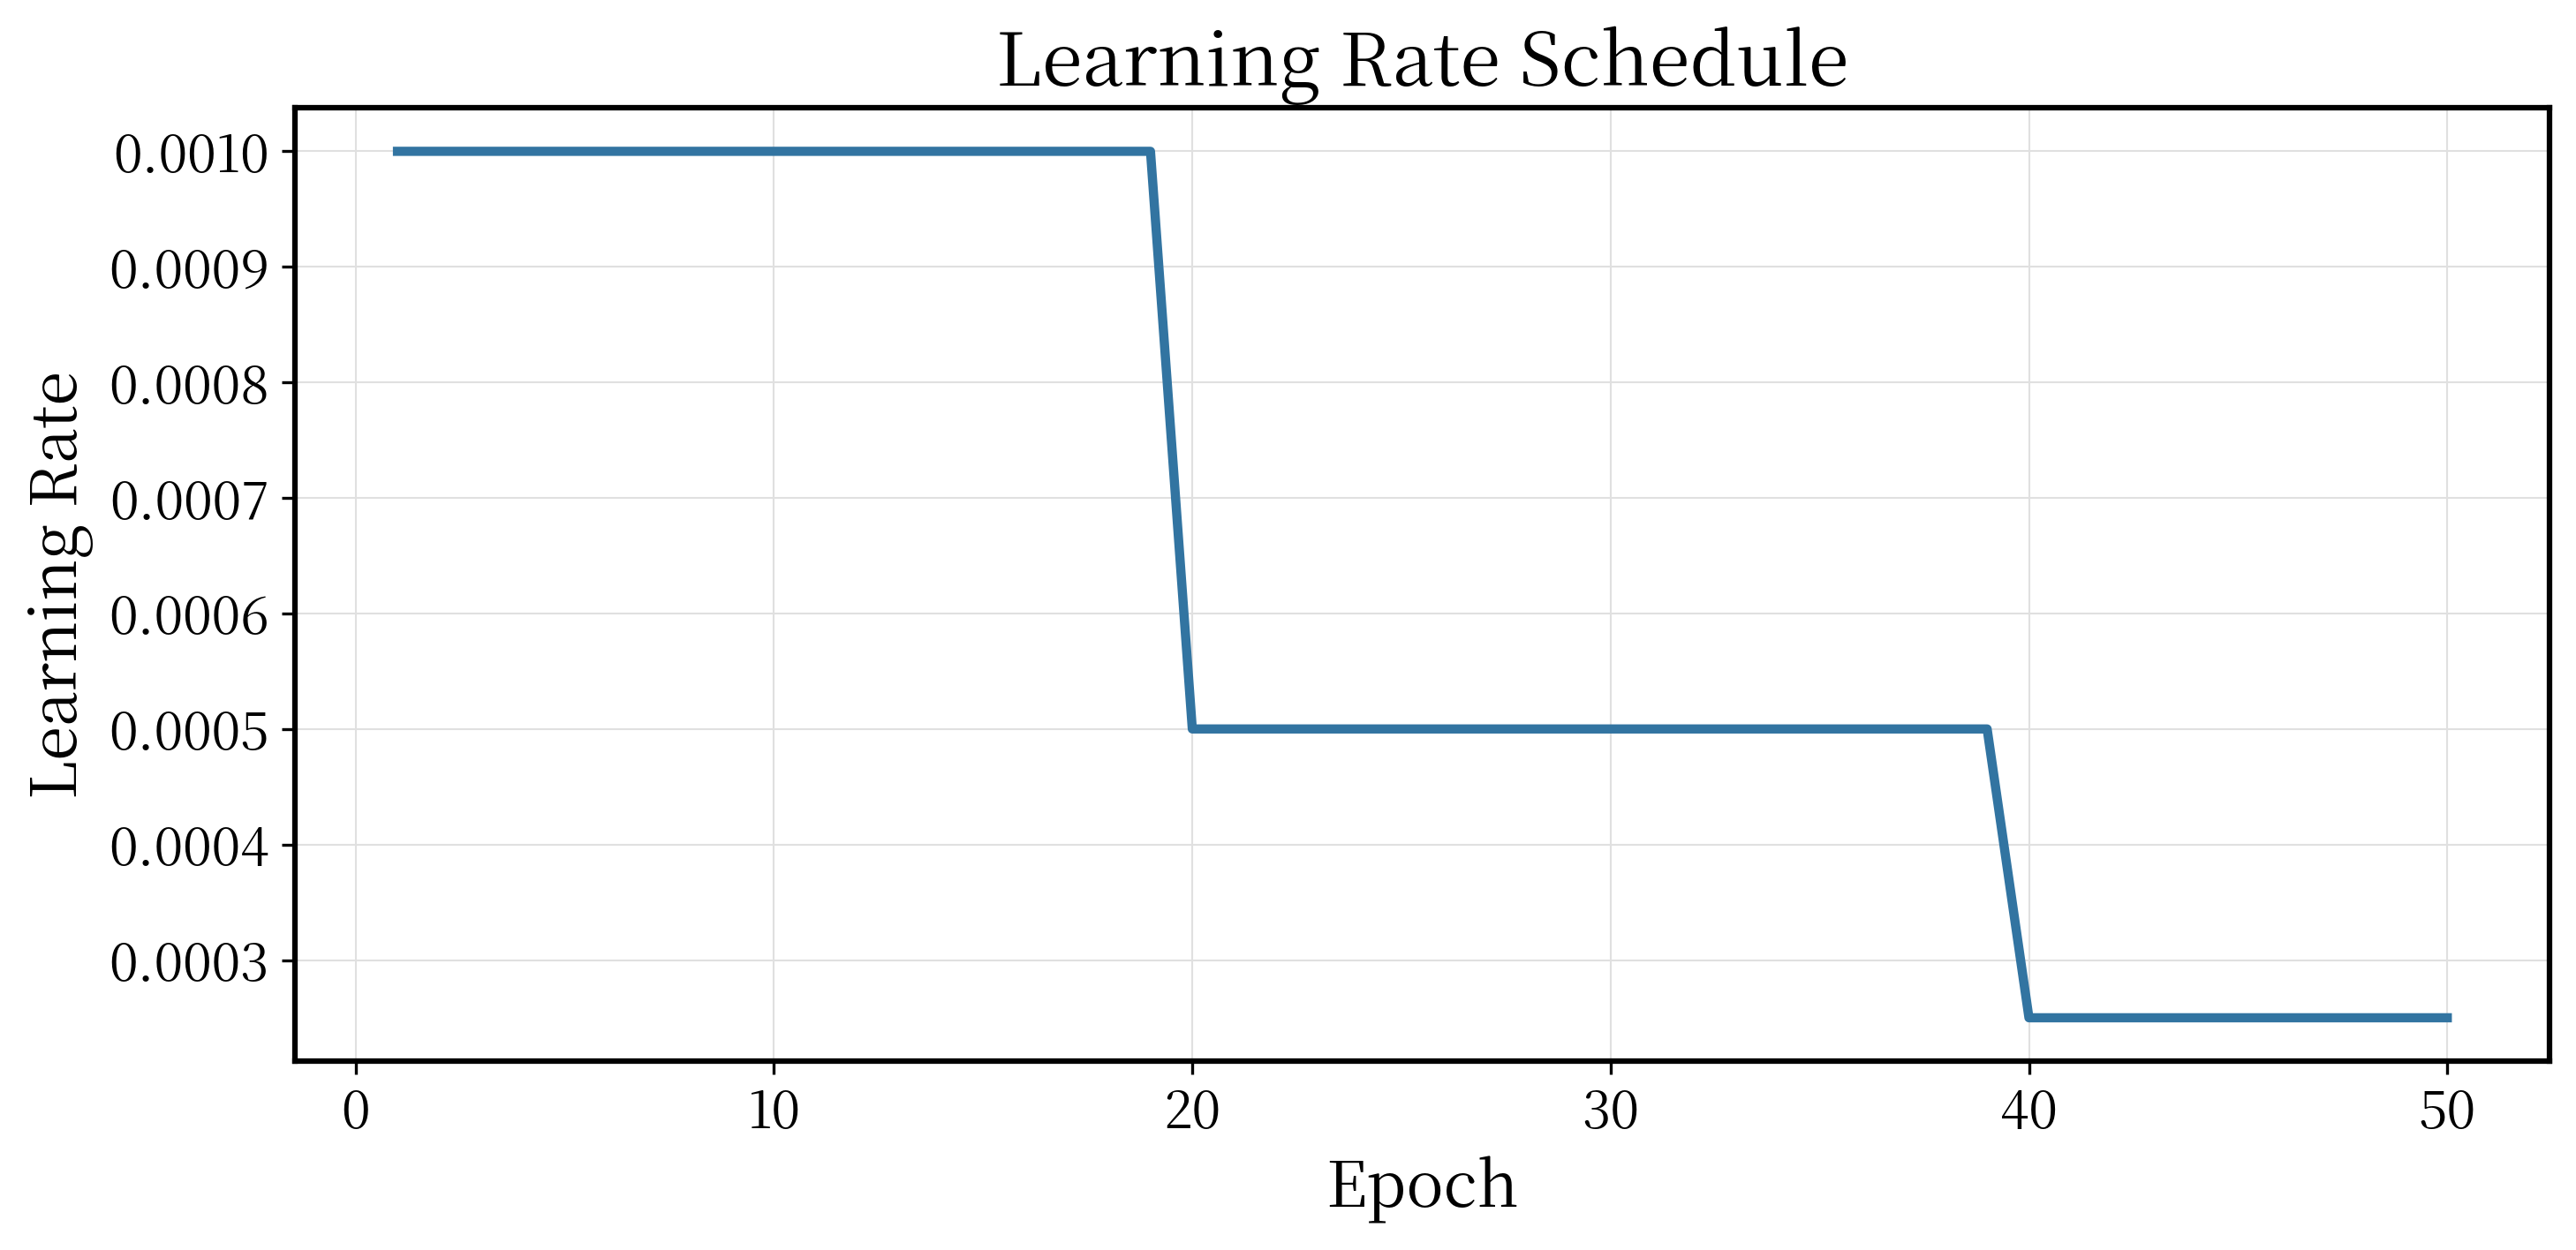
\includegraphics[width=0.8\textwidth]{figs/fig06_lr.png}
\caption{学习率调度曲线}
\label{fig:lr}
\end{figure}

图\ref{fig:time}记录了每个epoch的训练时间，平均约31.3秒/epoch，50个epoch的总训练时间约26分钟，表明SegNet在紧凑的模型设计下具有较高的计算效率。

\begin{figure}[H]
\centering
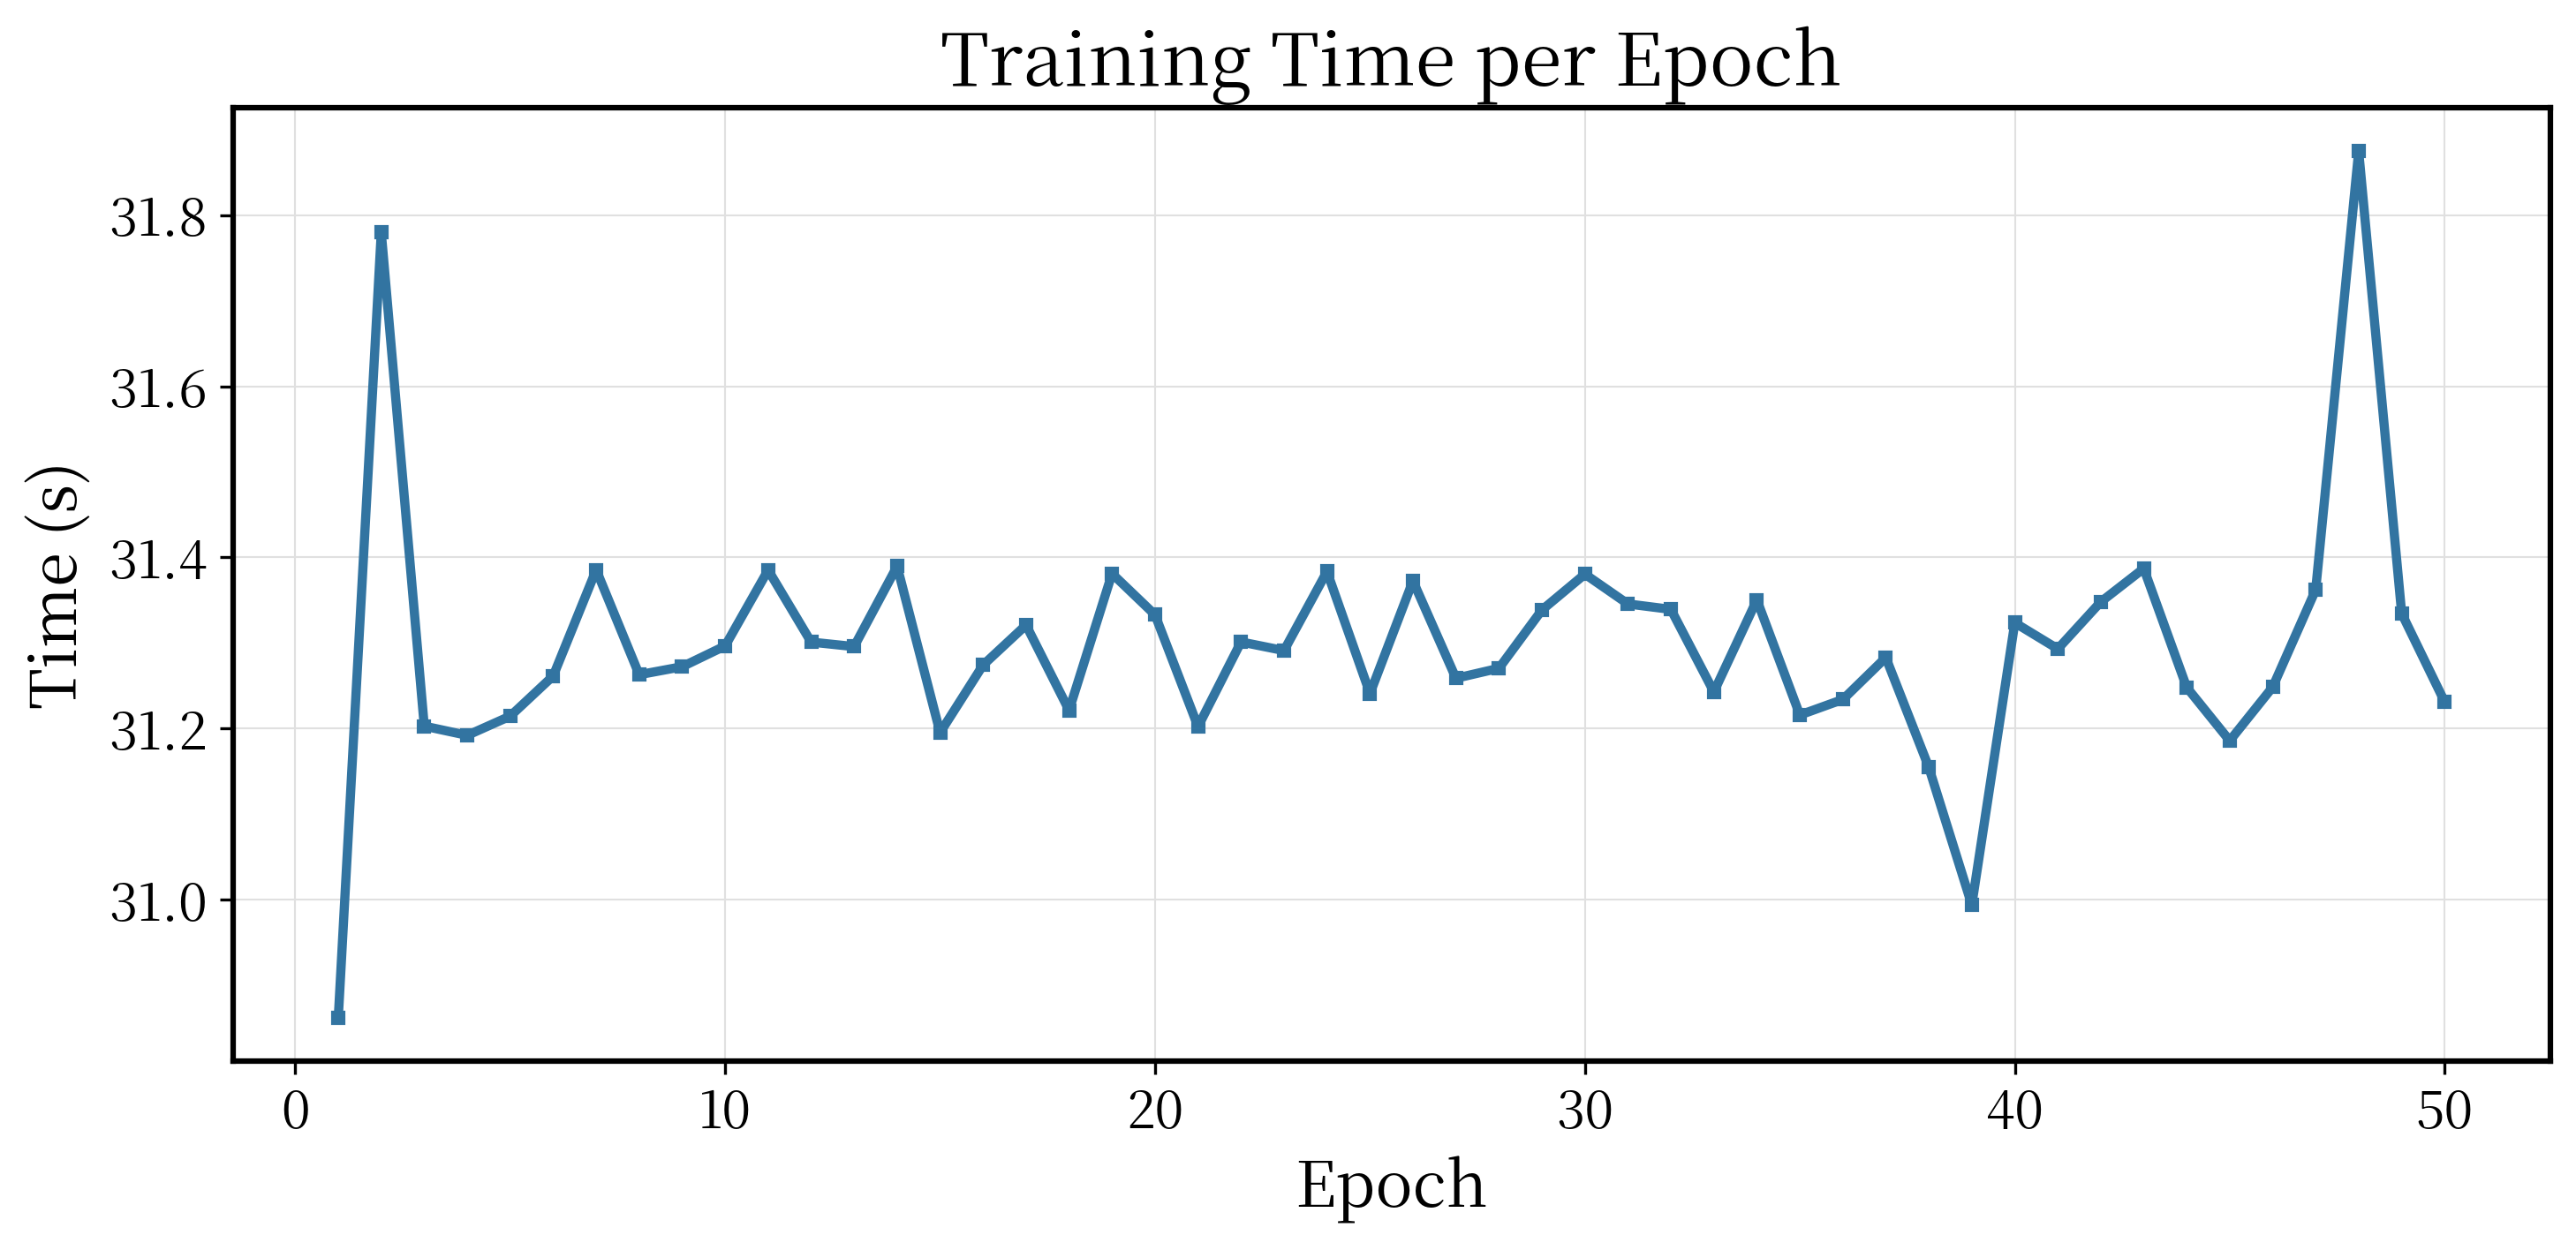
\includegraphics[width=0.8\textwidth]{figs/fig07_epoch_time.png}
\caption{每轮训练时间}
\label{fig:time}
\end{figure}

\subsection{测试集评估}

\begin{table}[H]
\centering
\caption{测试集最终评估结果}
\label{tab:test}
\begin{tabular}{lccc}
\toprule
\textbf{指标} & \textbf{Pixel Accuracy} & \textbf{mPA} & \textbf{mIoU} \\
\midrule
测试集 & 98.21\% & 96.93\% & \textbf{93.97\%} \\
验证集（最佳） & 99.48\% & 98.37\% & 96.94\% \\
\bottomrule
\end{tabular}
\end{table}

图\ref{fig:test}展示了模型在测试集上的最终评估结果。测试集上PA=98.21\%、mPA=96.93\%、mIoU=93.97\%，相比验证集有约3个百分点的mIoU下降，这属于正常范围内的泛化差距，说明模型并未严重过拟合到验证集的特定数据分布上。

\begin{figure}[H]
\centering
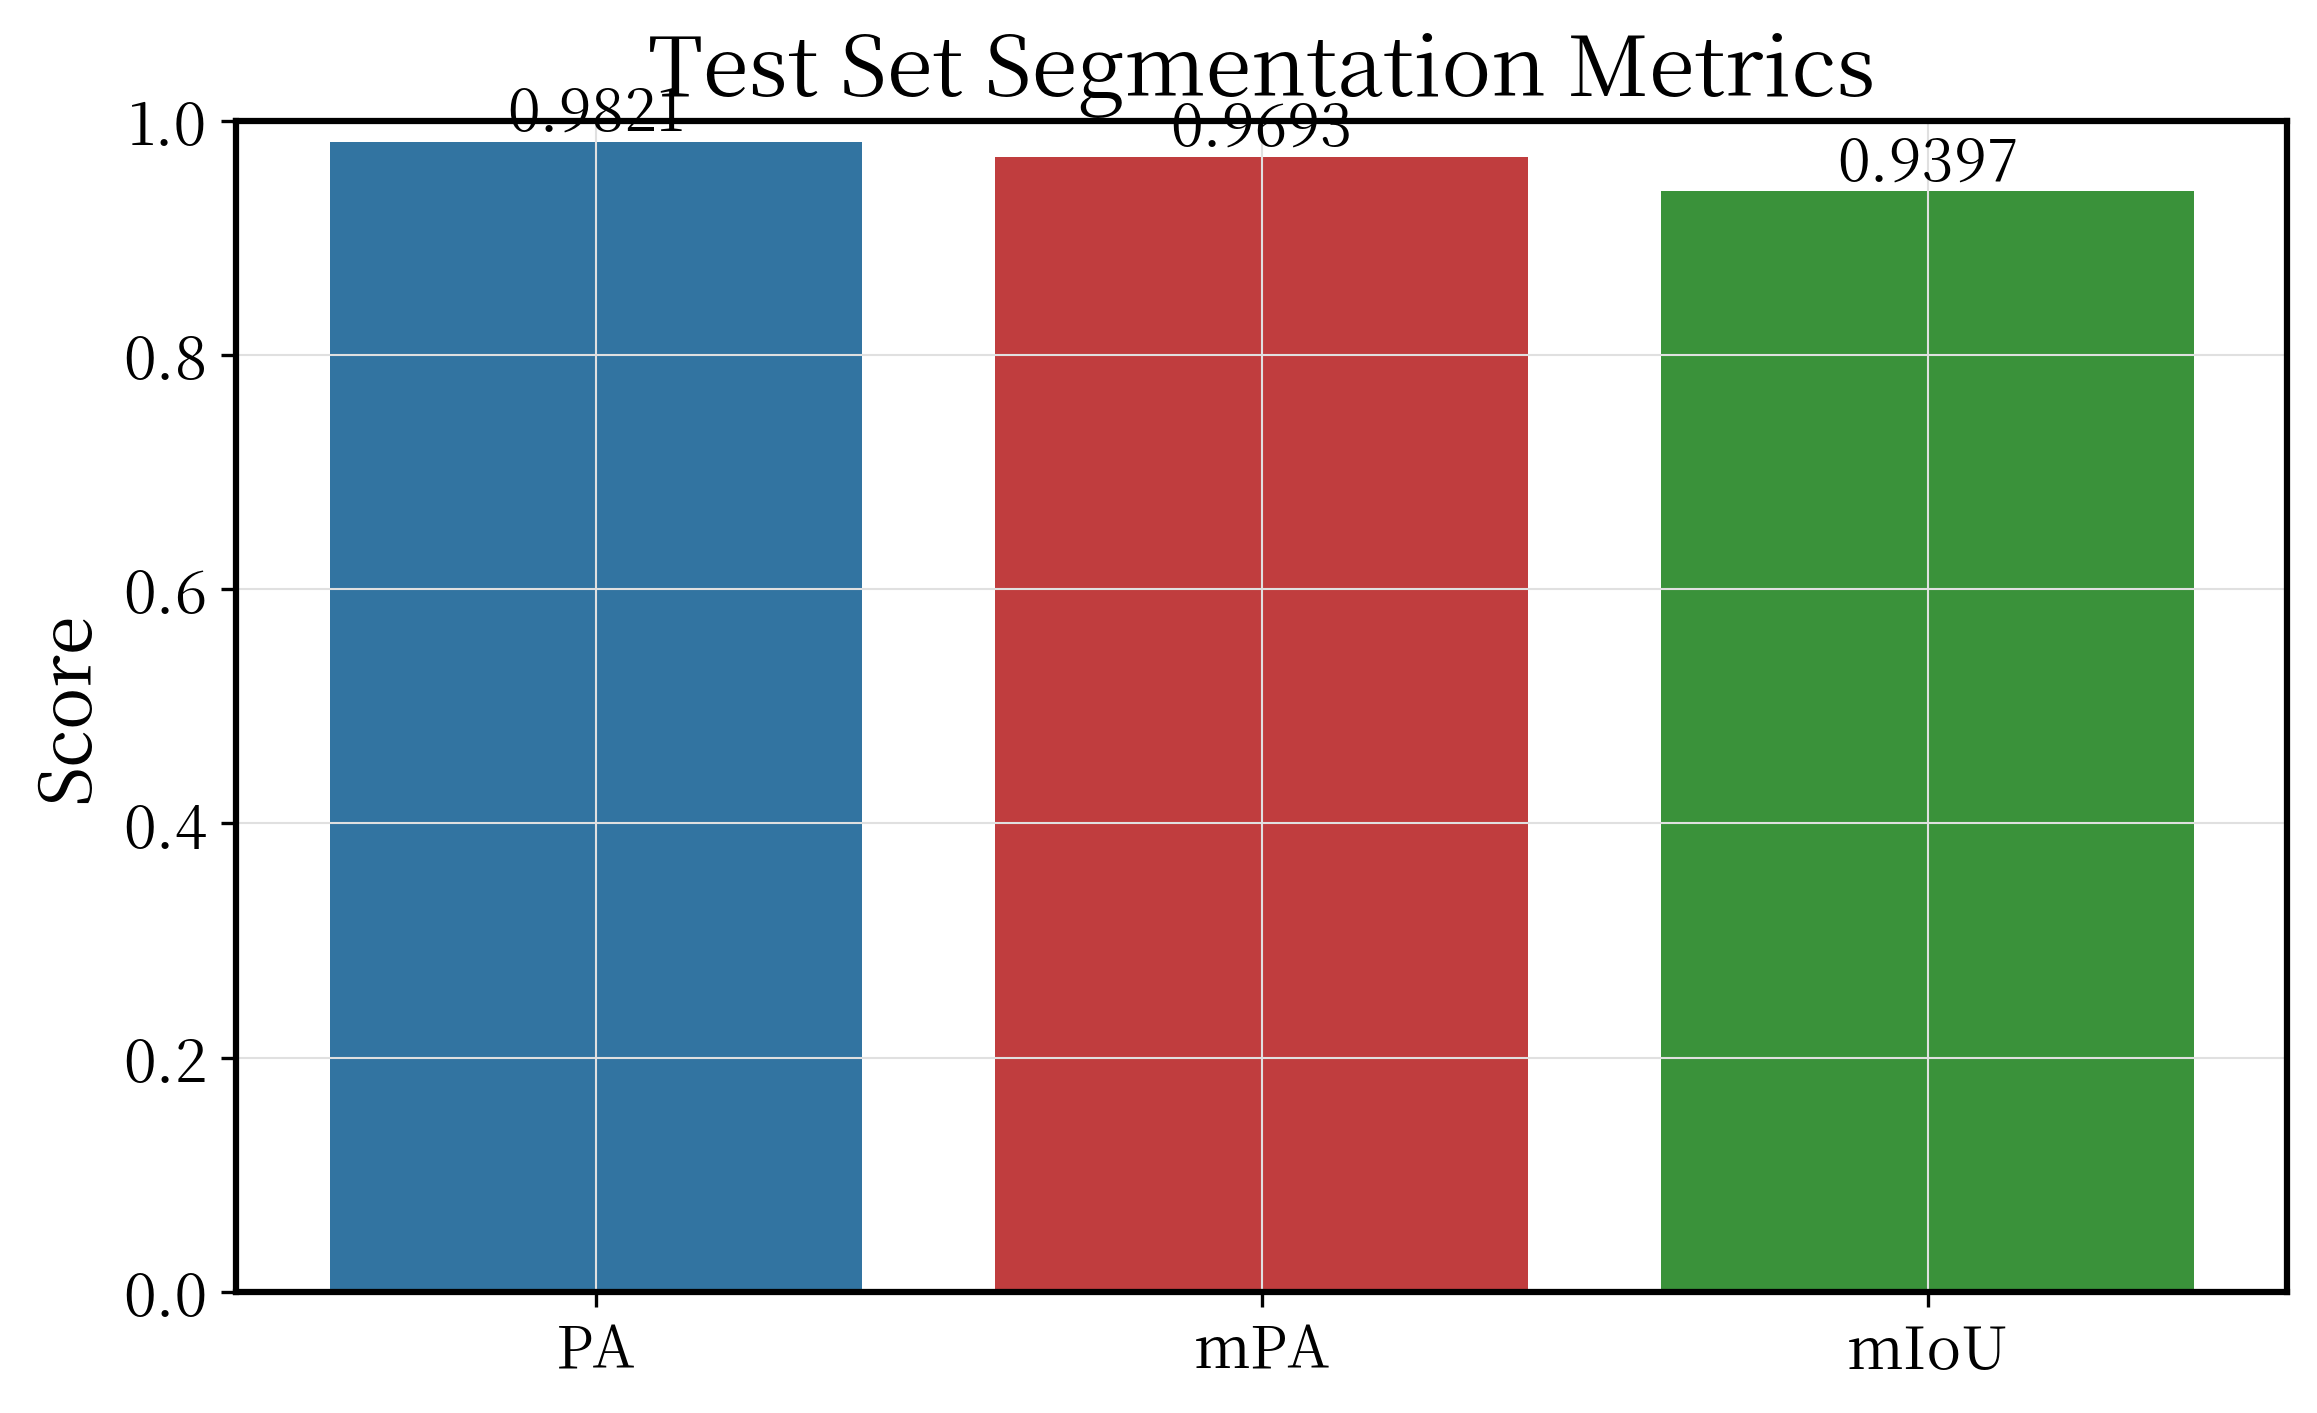
\includegraphics[width=0.8\textwidth]{figs/fig08_test_metrics.png}
\caption{测试集评估结果}
\label{fig:test}
\end{figure}

\section{深入讨论}

SegNet的池化索引上采样机制相比其他上采样方法具有独特优势。转置卷积虽然灵活但容易产生棋盘格伪影，双线性插值虽然平滑但丢失了空间位置信息，而池化索引能够精确地将特征恢复到池化前的位置，特别有助于保持目标边界的锐利度。然而，这种方法也有局限性：池化索引只保留了位置信息而丢弃了幅值信息，上采样后的特征图非常稀疏，完全依赖后续卷积层来填充和细化。

与U-Net的跳跃连接相比，SegNet的池化索引传递的信息量更少（仅有位置索引而非完整特征图），但所需的存储空间也更小。U-Net的跳跃连接直接将编码器的完整特征图与解码器特征拼接，提供了更丰富的多尺度信息，通常能取得更高的分割精度，但代价是推理时的内存占用显著增加。在自动驾驶等对实时性和内存有要求的场景中，SegNet的紧凑设计更具实用价值。

类别不平衡问题是影响分割性能的关键因素。实验中采用的加权交叉熵损失有效提升了稀有类别的分割质量——从测试集mIoU=93.97\%的结果来看，加权策略使模型在32个类别上都取得了合理的分割效果。进一步的改进可以引入Focal Loss或OHEM（Online Hard Example Mining）策略来更精细地关注困难样本。

\section{实验总结}

本实验成功实现了基于SegNet的街景语义分割任务，在CamVid数据集上经过50轮训练后，模型在测试集上达到了PA=98.21\%、mPA=96.93\%、mIoU=93.97\%的分割精度。通过实验深入理解了编码器-解码器架构的设计原理，特别是池化索引上采样机制相比转置卷积和双线性插值在边界保持上的优势。同时，实验中对类别不平衡问题的处理（加权交叉熵损失）、学习率多步衰减策略的选择等实践经验，为后续更高级的分割任务（如实例分割、全景分割）提供了重要的技术积累。

\end{document}
